\section{Fisher and Jeffreys: Two Roads Diverged in the Inference Forest}

\subsection{Probability Distributions and Estimation: What Can We Learn From Data?}

While Kolmogorov was busy laying the rigorous foundations of probability theory in the 1930s, other mathematicians were too busy inventing statistical methods to care. Chief among them: \textbf{Ronald Fisher} and \textbf{Harold Jeffreys}.

Their work wasn’t about axioms or measurable spaces—it was about solving real-world problems. How do you make sense of noisy data? How do you estimate unknown quantities? How do you make decisions under uncertainty?

Kolmogorov gave probability a foundation.  
Fisher and Jeffreys turned it into a toolkit.

At the heart of both men’s work was a new object: the \textbf{probability distribution}. Instead of assigning fixed values to outcomes, distributions model how likely different values are.

Suppose we measure the temperature of a sensor and assume it follows a normal distribution with unknown mean \( \mu \) and known standard deviation \( \sigma \). The key question: \textbf{How do we estimate \( \mu \) from the data?}


\begin{figure}[H]
\centering
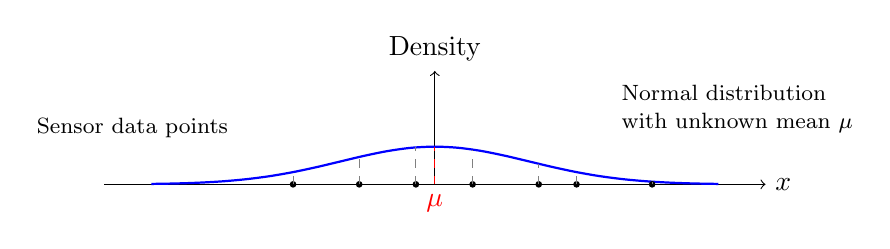
\begin{tikzpicture}[scale=1.2]
  % Axis
  \draw[->] (-3.5,0) -- (3.5,0) node[right] {$x$};
  \draw[->] (0,0) -- (0,1.2) node[above] {Density};

  % Normal distribution curve
  \draw[thick,domain=-3:3,smooth,variable=\x,blue] 
    plot ({\x},{exp(-(\x)^2/2)/sqrt(2*pi)});

  % True mean μ
  \draw[dashed,red] (0,0) -- (0,{exp(0)/sqrt(2*pi)});
  \node[below,red] at (0,0) {$\mu$};

  % Sample data points
  \foreach \x in {-1.5, -0.8, -0.2, 0.4, 1.1, 1.5, 2.3} {
    \fill[black] (\x,0) circle (1pt);
    \draw[gray, dashed] (\x,0) -- (\x,{exp(-(\x)^2/2)/sqrt(2*pi)});
  }

  % Annotation
  \node[align=left] at (3.2,0.8) {\footnotesize Normal distribution\\[-2pt] \footnotesize with unknown mean $\mu$};
  \node[align=center] at (-3.2,0.6) {\footnotesize Sensor data points};

\end{tikzpicture}
\caption{Estimating the mean \( \mu \) of a normal distribution from sensor data.}
\end{figure}


\begin{example}
Suppose we collect 10 temperature readings from a sensor:

\[
\{22.1, 21.8, 22.3, 21.9, 22.0, 21.7, 22.2, 22.1, 21.9, 22.0\}
\]

Assume the readings follow a normal distribution with known standard deviation \( \sigma = 0.2 \), but unknown mean \( \mu \). Our goal is to estimate \( \mu \).

\textbf{Fisher's Approach (Maximum Likelihood Estimation)}:  
We choose the value of \( \mu \) that maximizes the likelihood of observing the data. This leads to:

\[
\hat{\mu}_{\text{MLE}} = \frac{1}{n} \sum_{i=1}^{n} x_i = 22.0
\]

\textbf{Jeffreys' Bayesian View}:  
We treat \( \mu \) as a random variable and compute a posterior distribution over its possible values. Assuming a uniform prior for \( \mu \), the posterior is also normal:

\[
\mu \mid \text{data} \sim \mathcal{N}\left(\bar{x}, \frac{\sigma^2}{n}\right) = \mathcal{N}(22.0,\ 0.004)
\]

Here, Jeffreys gives us not just a point estimate, but a distribution reflecting our uncertainty about \( \mu \).

\textit{Interpretation}:  
Fisher gives us the most likely value; Jeffreys gives us a full picture of what we believe after seeing the data.
\end{example}

This simple example captures a deep philosophical divide: do we estimate fixed parameters, or reason about distributions over them? In the next sections, we’ll explore what this actually means—mathematically, computationally, and philosophically—as we dive deeper into likelihoods, priors, and the art of inference.







\subsection{The Estimator: Guessing the Unknown from What You Know}

Imagine you're trying to guess the average height of all the trees in a massive forest. You can’t measure every tree—there are millions. So instead, you walk around, measure a few, and try to make an educated guess.

This guess is called an \textbf{estimator}.

An estimator is a \textit{rule} or formula that takes your sample—the trees you actually measured—and uses it to guess something about the entire forest. You don't know the true average height (\( \mu \)), but based on your sample, you can compute the sample mean:

\[
\hat{\mu} = \frac{1}{n} \sum_{i=1}^n x_i
\]

Here, \( x_1, x_2, \dots, x_n \) are the tree heights you observed, and \( \hat{\mu} \) is your guess for the forest-wide average.

\begin{figure}[H]
\centering
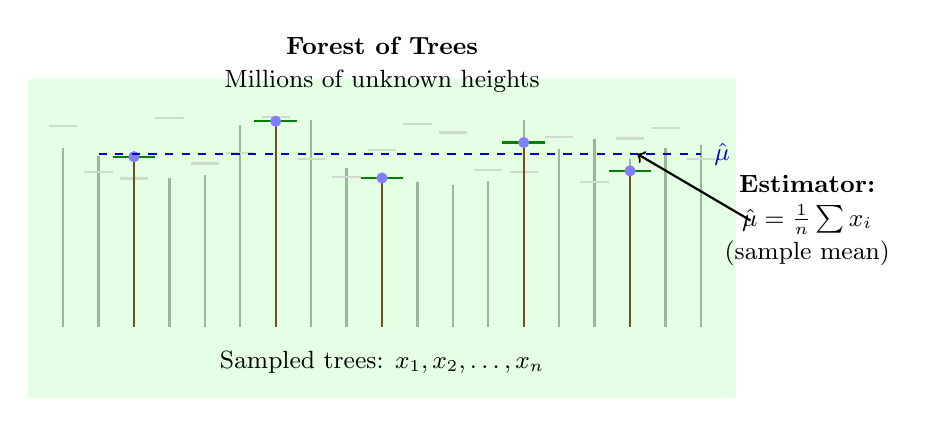
\begin{tikzpicture}[scale=0.9, every node/.style={font=\small}]

  % Forest background
  \fill[green!10] (-5,-1) rectangle (5,3.5);

  % Draw many trees in background (faint)
  \foreach \x in {-4.5,-4,...,4.5} {
    \draw[green!30!black!40, thick] (\x,0) --++ (0,2.5+rand*0.5);
    \draw[green!30!black!20, thick] (\x-0.2,2.5+rand*0.5) --++ (0.4,0);
  }

  % Highlighted sample trees
  \foreach \x/\h in {-3.5/2.4, -1.5/2.9, 0/2.1, 2/2.6, 3.5/2.2} {
    \draw[brown!60!black, thick] (\x,0) --++ (0,\h);
    \draw[green!50!black, thick] (\x-0.3,\h) --++ (0.6,0);
    \filldraw[blue!50] (\x,\h) circle (2pt);
  }

  % Sample mean line
  \draw[dashed,blue!80!black, thick] (-4,2.44) -- (4.5,2.44);
  \node[blue!80!black] at (4.8,2.44) {$\hat{\mu}$};

  % Label for sample
  \node at (0,-0.5) {Sampled trees: \( x_1, x_2, \dots, x_n \)};

  % Forest label
  \node[align=center] at (0,3.7) {\textbf{Forest of Trees}\\[1pt] Millions of unknown heights};

  % Estimator annotation
  \node[align=center] at (6,1.5) {\textbf{Estimator:}\\[1pt]
  \( \hat{\mu} = \frac{1}{n} \sum x_i \)\\[1pt] 
  (sample mean)};

  \draw[->, thick] (5.2,1.5) -- (3.6,2.44);

\end{tikzpicture}
\caption{Using a sample of tree heights to estimate the true forest-wide average.}
\end{figure}


\textbf{But—and this is crucial—your guess is still uncertain.} If someone else took a different path through the forest and measured different trees, they’d get a different \( \hat{\mu} \). That’s why an estimator isn’t just a number—it’s a \textit{random variable}. It depends on the data you happen to see.

\begin{quote}
An estimator is like a recipe. The data are the ingredients. You don’t know what you’ll cook up until the ingredients arrive.
\end{quote}

Statisticians care deeply about how good that recipe is. Does it tend to give the right answer on average? (That’s called \textbf{unbiasedness}.) Does it bounce around a lot from one sample to the next? (That’s \textbf{variance}.) And is it the best recipe possible under the circumstances? (That’s \textbf{efficiency}.)

Estimators are everywhere: polling results, risk scores, credit ratings, weather forecasts—they’re all just educated guesses, made from samples, trying to say something about a bigger, hidden world.

\begin{example}
Suppose we want to estimate the average number of hours students sleep per night at a university. We randomly sample 5 students and record their sleep hours:

\[
x = \{6.5, 7, 8, 5.5, 7.5\}
\]

We use the sample mean as our estimator:

\[
\hat{\mu} = \frac{1}{5}(6.5 + 7 + 8 + 5.5 + 7.5) = 6.9
\]

This is our estimate of the true average \( \mu \). But if we took another sample—say:

\[
x' = \{6, 6.5, 7.5, 6, 7\}
\]

—we’d get:

\[
\hat{\mu}' = \frac{1}{5}(6 + 6.5 + 7.5 + 6 + 7) = 6.6
\]

Same estimator, different data, different outcome. This variability is what makes the estimator a random variable.

If we repeatedly sampled and computed \( \hat{\mu} \) each time, the average of all those estimates would tend to converge to the true value \( \mu \). That’s why this estimator is \textbf{unbiased}. But those estimates would still vary from sample to sample—that’s the estimator’s \textbf{variance}.

\textit{Moral of the story:} A good estimator doesn’t just give a number—it gives a trustworthy guess, grounded in data but humble about uncertainty.
\end{example}






\subsection{Fisher’s World: Likelihoods and Information}

Fisher didn’t care about probabilities as degrees of belief. For him, probability was a model of how nature produces data. Once the data arrives, the job of statistics is to invert the process.

He introduced the \textbf{likelihood function}:

\[
\mathcal{L}(\theta) = P(\text{data} \mid \theta)
\]

This measures how likely a parameter \( \theta \) is to have generated the data. In Fisher’s world, the data is fixed and the parameter is unknown but \textit{not random}.

He also introduced the concept of \textbf{Fisher information}—a way to quantify how much information the data carries about the parameter:

\[
\mathcal{I}(\theta) = \mathbb{E}\left[ \left( \frac{\partial}{\partial \theta} \log P(X \mid \theta) \right)^2 \right]
\]

High Fisher information means sharper likelihoods—data that’s more decisive. This would go on to power everything from efficient estimators to the Cramér-Rao bound.

\begin{figure}[H]
\centering
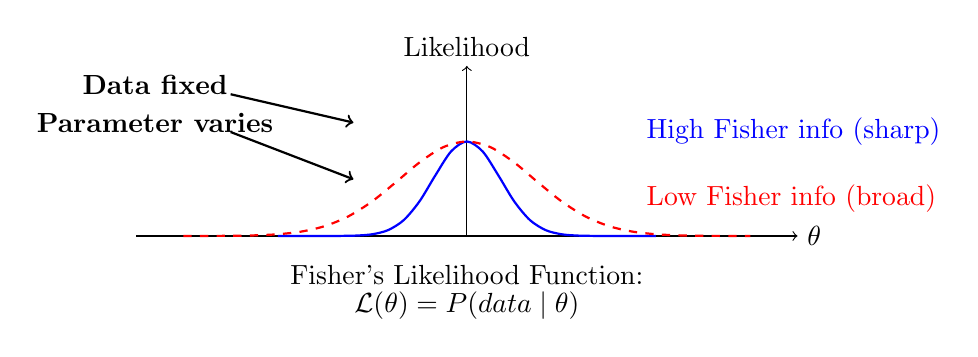
\begin{tikzpicture}[scale=1.2]
  % Axes
  \draw[->] (-3.5,0) -- (3.5,0) node[right] {$\theta$};
  \draw[->] (0,0) -- (0,1.8) node[above] {Likelihood};

  % High Fisher information (sharp peak)
  \draw[thick,blue,domain=-2:2,smooth,variable=\x] 
    plot ({\x},{exp(-4*(\x)^2)});

  % Low Fisher information (broad peak)
  \draw[thick,red,dashed,domain=-3:3,smooth,variable=\x] 
    plot ({\x},{exp(-(\x)^2)});

  % Labels
  \node[blue,right] at (1.8,1.1) {High Fisher info (sharp)};
  \node[red,right] at (1.8,0.4) {Low Fisher info (broad)};

  % Data fixed arrow
  \node at (-3.3,1.6) {\textbf{Data fixed}};
  \draw[->, thick] (-2.5,1.5) -- (-1.2,1.2);

  % Parameter θ varies arrow
  \node at (-3.3,1.2) {\textbf{Parameter varies}};
  \draw[->, thick] (-2.5,1.1) -- (-1.2,0.6);

  % Annotation
  \node[align=center] at (0,-0.6) {
    Fisher’s Likelihood Function: \\[-2pt]
    \( \mathcal{L}(\theta) = P(\text{data} \mid \theta) \)
  };

\end{tikzpicture}
\caption{In Fisher’s view, data is fixed and the likelihood is a function of the parameter \( \theta \). The sharper the peak, the more information the data carries about \( \theta \).}
\end{figure}


\subsubsection{A Worked Example: Likelihood and Fisher Information in Action}

Imagine you're studying radioactive particles, and you're measuring how long they take to decay. These decay times are unpredictable, but they follow a well-known pattern: the exponential distribution.

\[
f(x \mid \lambda) = \lambda e^{-\lambda x}, \quad x \geq 0
\]

Here, \( \lambda \) is the decay rate—how quickly things fall apart. And you're trying to estimate it from data. But you’ve only seen one decay event, and it happened at exactly \( x = 2 \) seconds.

\begin{figure}[H]
\centering
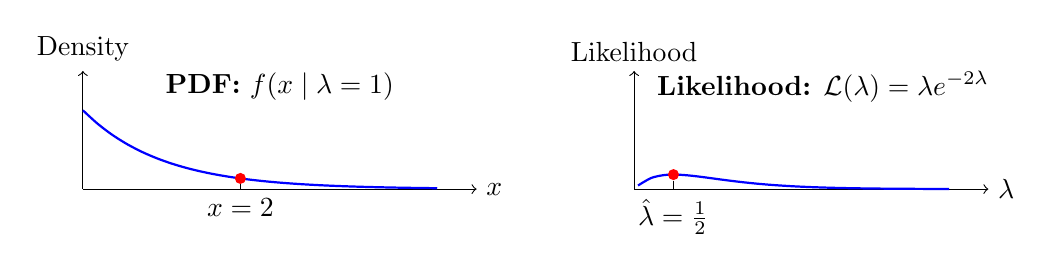
\begin{tikzpicture}

% Left plot: Exponential PDF with fixed lambda
\begin{scope}[scale=1]
  % Axes
  \draw[->] (0,0) -- (5,0) node[right] {$x$};
  \draw[->] (0,0) -- (0,1.5) node[above] {Density};

  % Exponential curve for lambda = 1
  \draw[thick,blue,domain=0:4.5,smooth,variable=\x] 
    plot ({\x},{exp(-\x)});

  % Mark x = 2
  \draw[dashed] (2,0) -- (2,{exp(-2)});
  \fill[red] (2,{exp(-2)}) circle (2pt);
  \node[below] at (2,0) {$x = 2$};

  % Label
  \node at (2.5,1.3) {\textbf{PDF:} \( f(x \mid \lambda = 1) \)};
\end{scope}

% Right plot: Likelihood as function of lambda
\begin{scope}[xshift=7cm,scale=1]
  % Axes
  \draw[->] (0,0) -- (4.5,0) node[right] {$\lambda$};
  \draw[->] (0,0) -- (0,1.5) node[above] {Likelihood};

  % Likelihood curve: L(lambda) = lambda * exp(-lambda * 2)
  \draw[thick,blue,domain=0.05:4,smooth,variable=\l] 
    plot ({\l},{\l*exp(-2*\l)});

  % Peak of the likelihood (at 1/2)
  \draw[dashed] ({1/2},0) -- ({1/2},{(1/2)*exp(-1)});
  \fill[red] ({1/2},{(1/2)*exp(-1)}) circle (2pt);
  \node[below] at (0.5,0) {$\hat{\lambda} = \frac{1}{2}$};

  % Label
  \node at (2.4,1.3) {\textbf{Likelihood:} \( \mathcal{L}(\lambda) = \lambda e^{-2\lambda} \)};
\end{scope}

\end{tikzpicture}
\caption{Left: PDF of exponential decay with \( \lambda = 1 \). Right: Likelihood of \( \lambda \) given observed decay at \( x = 2 \). The peak occurs at \( \hat{\lambda} = 1/2 \).}
\end{figure}


\vspace{0.5em}
\noindent
\textbf{Step 1: Likelihood—What Would Make This Observation Most Expected?}

The likelihood function tells you: if you assume a particular value of \( \lambda \), how plausible is it that you’d see a decay at 2 seconds?

\[
\mathcal{L}(\lambda) = \lambda e^{-2\lambda}
\]

This is like playing a game of “Guess the Parameter” where each guess gets a score based on how well it explains what you saw. The best guess—the one that makes your observation most likely—is the peak of this curve.

It turns out this peak is at:

\[
\hat{\lambda}_{\text{MLE}} = \frac{1}{2}
\]

So based on that one event at 2 seconds, your best guess is that the true decay rate is 0.5. Not certain—just most likely.


\begin{figure}[H]
\centering
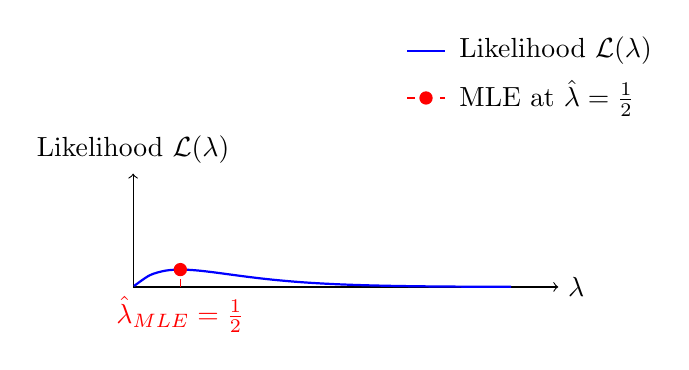
\begin{tikzpicture}[scale=1.2]

  % Axes
  \draw[->] (0,0) -- (4.5,0) node[right] {$\lambda$};
  \draw[->] (0,0) -- (0,1.2) node[above] {Likelihood \( \mathcal{L}(\lambda) \)};

  % Likelihood curve: L(lambda) = lambda * exp(-2*lambda)
  \draw[thick,blue,domain=0.01:4,smooth,variable=\l] 
    plot ({\l},{\l*exp(-2*\l)});

  % Peak at lambda = 0.5
  \draw[dashed,red] (0.5,0) -- (0.5,{0.5*exp(-1)});
  \fill[red] (0.5,{0.5*exp(-1)}) circle (2pt);
  \node[below,red] at (0.5,0) {\( \hat{\lambda}_{\text{MLE}} = \frac{1}{2} \)};

  % Legend box
  %\draw[fill=white, draw=black] (2.8,0.1) rectangle (4.2,0.6);

  % Legend entries
  \draw[thick,blue] (2.9,2.5) -- (3.3,2.5);
  \node[right] at (3.35,2.5) {Likelihood \( \mathcal{L}(\lambda) \)};

  \draw[red,dashed] (2.9,2) -- (3.3,2);
  \fill[red] (3.1,2) circle (2pt);
  \node[right] at (3.35,2) {MLE at \( \hat{\lambda} = \frac{1}{2} \)};

\end{tikzpicture}
\caption{The likelihood function \( \mathcal{L}(\lambda) = \lambda e^{-2\lambda} \). The peak at \( \lambda = \frac{1}{2} \) is the MLE: the parameter value that makes observing a 2-second decay most plausible.}
\end{figure}




\vspace{0.5em}
\noindent
\textbf{Step 2: Fisher Information—How Sharp Is Your Guess?}

Fisher Information measures how much information your observation gives you about the parameter. In a way, it’s a sensitivity check: if small changes in \( \lambda \) make big changes in likelihood, then your data is highly informative. If the likelihood curve is flat and squishy, your data doesn’t help much.

For the exponential distribution, the Fisher information for one observation is:

\[
\mathcal{I}(\lambda) = \frac{1}{\lambda^2}
\]

Here’s what that means:

\begin{itemize}
    \item If \( \lambda = 0.5 \), then \( \mathcal{I} = 4 \): you get a sharp, confident estimate.
    \item If \( \lambda = 2 \), then \( \mathcal{I} = 0.25 \): the estimate is fuzzier.
\end{itemize}

\vspace{0.5em}
\noindent
\textbf{Conclusion:} When decay is slow, each observation is packed with information—you can see more of the “tail” of the distribution. But when decay is fast, it’s harder to learn anything from one quick blip. The Fisher information puts numbers on this intuition.






\begin{figure}[H]
\centering
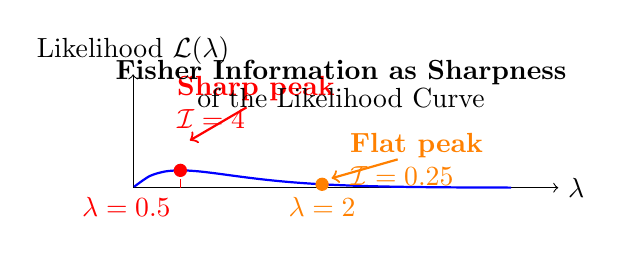
\begin{tikzpicture}[scale=1.2]

  % Axes
  \draw[->] (0,0) -- (4.5,0) node[right] {$\lambda$};
  \draw[->] (0,0) -- (0,1.2) node[above] {Likelihood \( \mathcal{L}(\lambda) \)};

  % Likelihood curve for x=2: L(lambda) = lambda * exp(-2*lambda)
  \draw[thick,blue,domain=0.01:4,smooth,variable=\l] 
    plot ({\l},{\l*exp(-2*\l)});

  % Highlight lambda = 0.5 (sharp)
  \draw[dashed,red] (0.5,0) -- (0.5,{0.5*exp(-1)});
  \fill[red] (0.5,{0.5*exp(-1)}) circle (2pt);
  \node[below left,red] at (0.5,0) {\( \lambda = 0.5 \)};
  \node[red,align=left] at (1.3,0.9) {\textbf{Sharp peak}\\\(\mathcal{I} = 4\)};
  \draw[->,red,thick] (1.2,0.85) -- (0.6,0.5);

  % Highlight lambda = 2 (flat)
  \draw[dashed,orange] (2,0) -- (2,{2*exp(-4)});
  \fill[orange] (2,{2*exp(-4)}) circle (2pt);
  \node[below,orange] at (2,0) {\( \lambda = 2 \)};
  \node[orange,align=left] at (3,0.3) {\textbf{Flat peak}\\\(\mathcal{I} = 0.25\)};
  \draw[->,orange,thick] (2.8,0.3) -- (2.1,0.1);

  % Title label
  \node[align=center] at (2.2,1.1) {
    \textbf{Fisher Information as Sharpness}\\[-2pt]
    of the Likelihood Curve
  };

\end{tikzpicture}
\caption{Sharper likelihoods (e.g., at \( \lambda = 0.5 \)) imply more Fisher information. Flatter likelihoods (e.g., at \( \lambda = 2 \)) imply less. Fisher information quantifies how much your data narrows down the parameter.}
\end{figure}



